\chapter{Character Creation}

Once you are happy with your worlds' settings, you now can select one of different game modes to start out with. This guide will focus on the [Custom Character] selection. Once selected and the content mods are all loaded into the system, not throwing any exceptions, you are brought to the character creation screen, separated into many different categories. First you are asked to select your point pool system: Multiple Pools, Single Pool or Freeform. Multiple Pools force you to use points in their respective pools or followup pools (except for skills). So you can't just pick a bunch of negative traits and rack up the attributes. Single Pool removes these limitations and you a free to use the points at your disposal to how you see it fit. Freeform is basically a cheat mode, you can use however many points you wish. For this Tutorial, we are going with Multiple Pools.

\section{Scenarios}

Once you have made your decision, you can choose a specific scenario that you are playing. These limit you in the terms of where you spawn, as what profession you can spawn, as well as imposing certain possibilities in the trait selection and potentially coming with extra merits that need to be resolved.

I highly suggest for a newcomer to use the Evacuee scenario and staying as far away as possible from any of the 'Challenge' scenarios. Those are meant for brutally difficult runs that are each challenging in their own rights and are no fun if you have next to no clue what you are doing. For the sake of this Tutorial, we will start as an Evacuee, but some other interesting starting Scenarios also include Wilderness, Sheltered (this is a winter spawn, regardless of season settings) or Refugee.

\section{Professions}

Professions in Cataclysm: Dark Days Ahead are what you'd consider to be your background. They either cost a certain amount of points to select, or give you points in return for selecting them. From a simple no name person, up to a hunter, blacksmith or mechanic, the variety is what nails it. Every background spawns with specific items and skills that they start out their journey with. While some come with handy tools to use, great skills for their cost, some are just more challenging because of what they don't come with. Some professions spawn with not only less of a certain thing, like clothes, but also come with negatives, such as addictions to certain drugs that will severely hamper your start (I'm specifically looking at you Tweaker!). Or some might be what you consider to be powerful cyborgs that come outfitted with Bionic implants (more on that later) that can greatly change the flow of the game - in a positive as well as negative direction. Professions can however, be locked behind certain starting scenarios or be excluded from some scenarios you'd consider them to be a part of. Feel free to check out the different scenarios' starting professions. As for this guide, I assume the profession of the Survivor, the most basic of the starts available.

This leaves us with 6 Stat points, 0 Trait points and 2 Skill points for our character creation for a total of 8.

\section{Traits}

Traits are the defining, well, traits that make you who you are: A faceless, nameless git that somehow managed to survive the initial strike of the cataclysm.

Traits can affect your gameplay in a positive or negative way in many different severities. (Specific professions get a 3rd tab, profession Traits, that is unavailable to most of the characters)

While traits may seem like something you can easily gloss over, they are however extremely important when it comes to how you want to experience the game.

Here I am going to give a quick list of traits (positive and negative) that I feel are worth picking up for several reasons:

\subsection{Positive Traits}

\textbf{Animal Empathy} (1 point) - smaller game is less likely to run away from you, while bigger animals like dogs, wolves or moose are less likely to just charge at you and attack. And believe me, moose are well-known early game character killers. So if you have the point to spare and trouble surviving in the wilderness, consider picking this up.

\textbf{Deft} (1 Point) - For those melee focused characters, being able to recover from a missed swing quicker means the enemy has less time to land a hit on you. Many Weapon- and Martial Arts style come with built-in deft like abilities, so it's not something one would be picking normally, but for those that neither have access or want to avoid special weapon styles, it can be worthwhile picking up.

\textbf{Disease Resistant} (1 Point) - While this will only save you from the more common diseases like the flu or the common cold, being more resistant to those in particular can be great if you happen to catch one of those more often than you'd like. Limited in usefulness in general, as ailments for those illnesses are commonplace. Consider it for a wilderness run - Bee Balm tea only gets you so far after all.

\textbf{Fast Healer} (2 Points) - You heal damage done to your body more quickly by sleeping, you even heal very small amounts of HP while awake and limbs will heal noticeably quicker. If you feel yourself taking damage a lot, which in turn leaves you crippled in your hideout, you might want to consider grabbing this trait.

\textbf{Fast Learner} (3 Points) - This will make all practically earned experiences raise your skills quicker. For the amount of points it costs, the effect it has is quite low. This does exclude knowledge gained from books, has however great application when training combat focused skills, as those will rise quicker, which makes for an easier life all around by quickly gaining combat related skill levels.

\textbf{Quick} (3 Points) - This makes you 10\% quicker in every aspect. From walking/running, to attacking, eating and whatnot. If you require that extra bit of performance from your character and have the points to spare, this is a great pick.

\textbf{Fast Reader} (1 Point) - Reading books that will provide you will extra skills far quicker than getting into fist-fights all the time? Definitely a nice pick if you want to learn most of your skills from books. Remember though, for combat related skills - books only get you so far as there are no end-game books for combat skills by design. The reading time on some late game books however might just make this trait worth the single point.

\textbf{Fleet-Footed} (2 Points) - Feeling a bit slow in comparison to the undead? Grab this perk to be 15\% quicker while on sure footing, which relates to all things you don't require to balance upon, like boulders, railings, rubble and wreckages.

\textbf{High Adrenaline} (2 Points) - This perk is more of a double-edged sword than one would believe. In tense combat moments you will gain the Adrenaline Rush effect, which boosts your Str, Dex and Per, as well as numbing pain a bit, while giving you great stamina recovery. However, once it wears off it leaves you pretty vulnerable as it does reduce your stats for a time. Take at your own risk - the power boost may save your bacon.

\textbf{Martial Arts Training, Melee Weapon Training, Self Defense Classes, Shaolin Adept and Venom Mob Protegee} (2 to 3 points each) - What all of those traits have in common is that these traits (more like backgrounds or hobbies) will provide you with 1 of the several different Martial Arts and Weapon Arts the game has to offer. These will drastically change combat capabilities and can turn the tide in many of the different combat scenarios you may find yourself in. Anybody wanting to play a martial artist is bound to pick one of those, as a no-style unarmed combat characters' damage is significantly lower

For those that wish to become really strong early on. I'd suggest Melee Weapons Training (Eskrima) and grabbing yourself a pipe to smack enemies around with.

For a more in-depth look at the respective Martial Arts, I can only suggest you to check out this discourse post made:

https://discourse.cataclysmdda.org/t/best-unarmed-styles-for-early-game/15558/11

\textbf{Night Vision} (2 Points) - In my opinion an absolutely mandatory pick for any survivor out there. What this trait allows for is taking your perception and giving you 1 tile of vision for each 3 points in Perception while in complete darkness. This trait will NOT however allow you to do crafting that requires you to see or reading.

\textbf{Packmule} (2 points) - This perk will raise your volume capacity by 40\%. This does not include weight, which is covered by Strong Back (35\% more carry weight). This makes the most use out of all your pockets if you wish to travel in light gear and without a Backpack to keep your encumbrance low (more on encumbrance in chapter 4.2.2 - Temperature and Clothing) and is a definite pick for those that either wish to carry around some utility gear while also being clothed sparingly, or for the absolute hoarder that runs without a shopping cart.

\textbf{Parkour Expert} (2 Points) - Removes or lowers the movement penalty when moving through tiles that would slow you down. Railings, windows, bushes, grass, you name it. This allows you to widen the gap between you and monsters more easily. Makes for a great way of escaping, as well as a nice way to kite monsters into tiles that would slow them down, giving you more time to strike them

\textbf{Pain Resistant} (2 Points) - What is Pain? It's the reason you constantly die. Pain slows you down, which in relative terms, speeds up your enemies and allows them to get more hits in, it reduces your attributes quickly, sometimes drastically and it makes you miss more often in combat, which is the last thing you want while being so close to killing that last enemy. If you happen to be in pain quite often and Aspirin isn't doing it for you, consider picking this perk up to supplement it.

\textbf{Psychopath} (2 Points) - No guilt from killing enemies that you'd consider having scruples for. This means that killing zombie children and the likes will incur no penalty to your mood, which can quickly cripple your crafting capabilities. The perk has also the added benefit of you not caring about human life and allows you to freely kill, butcher, and eat human entities - a great extra food source.

\textbf{Robust Genetic} (3 points) - For those that wish to be more explorative with the inner workings of their body, this trait will make it so that mutations you receive either from outside influences (radiation, enemy attacks) or from willingly taking mutagens have a higher chance of being positive than negative. A must have for those that wish to play with mutations more.

\textbf{Strong Stomach} (1 Point) - This will keep your food down if you are nauseous from either drinking unclean water, which can poison you, or if you happen to get poisoned by an enemy. Works well in conjunction with the negative food traits.

\subsection{Negative Traits}

\textbf{Addictive Personality} (+2 Points) - Addictions will hit in quicker for you, and you'll have a harder time of getting rid of them. Sounds nasty, but if you use addictive items sparingly, like the odd cigarette, or not snort meth like it's nobody's business, you are totally fine with this perk. For those interested - you'd need to take in 3 doses and be unlucky enough to get 3 addiction level increases (more on that in Chapter 6.3.1)

\textbf{Animal Discord} (+1 Point) - if, on the other hand, animal life is not much of a threat to you since you know what you are doing, picking up animal discord can actually be a benefit, as it will make wild game more aggressive and therefore run away less often, helping you out while hunting small and big game alike.

\textbf{Far/Near-sighted} (+2 Points each) - glasses are extremely common in the apocalypse, and they are also quite sturdy, so having these traits is a total non-issue for the most part. Just make sure to not take them off, as Near-sighted limits your view range dramatically, while Far-sighted prevents you from reading and using Terminals and makes hitting things in combat pretty difficult. Also guarantees you to spawn with the appropriate set of glasses when you start out.

\textbf{Forgetful} (+3 Points) - Forgetful causes you to lose skills due to skill rust quicker and you will forget what map tiles are what when you are far away from them for extended time. If you play with skill rust disabled, the first effect won't work and therefore gives you basically 3 free points. Even with skill rust enabled, the effect is not too terrible. (I'd suggest playing with int-capped skill rust for best effect)

\textbf{Glass Jaw} (+2 Points) - while having less HP on your head seems to be a pretty nasty effect, remember that helmets of many different types are pretty common inside towns, and with some tailoring you are able to craft headgear which can be pretty powerful relatively early. If you feel daring, feel free to grab this perk for some extra points.

\textbf{Topographagnosia} (rolls right off your tongue) (+5 Points) - said to lower your vision on the overmap, this trait doesn't prevent map exploration through events. Checking the console for the Refugee Center will still show you most of the landmarks on the way for example. If your big worry is early game, this doesn't seem like it will hurt you too much while also giving a ridiculous amount of points in return.

\textbf{Trigger Happy} (+1 Point) - weapons that support full auto can rarely go full auto when firing. Not only does this not apply if you aren't using firearms that don't support full auto, if you intend to not use firearms at all, or in extremely bad situations (where Full auto might save your bacon) this trait is a safe pick

\textbf{Ugly and Truth teller} (each +1 Point) - negative NPC Traits - If you plan to not play with NPCs, again, free points. Even when playing with NPCs, lying is too difficult without any skill in speaking and being ugly only lowers the chances of talking down NPCs or asking them for equipment/skill training. This in itself can easily overcome by reading Book 'Self-Esteem for dummies' (speaking to 3) which is rather common.

\textbf{Slow/Very Slow/Extremely Slow Sleep healing} - as of Version 8211, these have been renamed to Slow Healer, Poor Healer, Imperceptive Healer (+2/4/8 Points) - depending on how much you enter combat and on how careful you tackle said combat, these traits can be rather helpful. Especially the Poor Healer perk seems to be a solid pickup since the most apparent effect is the slower sleep healing, which can be supported by makeshift bandages (free first aid training!). Beware however, as this trait-line WILL decrease the rate at which broken limbs mend respectively, and it can be extremely crippling to wait several days or weeks longer for a limb to be fixed. Again, pick only if you dare.

\subsection{Perks to avoid}
These perks I consider to be too low to be worth considering for various reasons. Either because the application is too limited at all, the benefits too small, or even hurtful in a way you aren't even expecting.

\paragraph{Positive:}

The NPC Perks - \textbf{Pretty, skilled liar} (-1 Point each) - like the negative traits, the effects gained from them are too small to be worthwhile. With the notable exception being that the negatives provide you with points, while with these, you'd waste them more often than not.

\textbf{Self-Aware} (-1 Point) - While this perk allows you to better gauge your general condition by letting you see the exact number of HP of each limb, the current Pain level as a numeric number, as well as your health stat (more on that later), the effect seems to be too weak overall to justify taking that 1 point off.

\textbf{Outdoorsman} (-1 Point) - while being wet carries a nasty debuff, it is also clearable by carrying a towel and using that to dry yourself off from said rain or wearing protective gear like a raincoat + hood for extended periods of work. Considering that staying wet makes it easy to catch the flu/cold, forgetting to do so after a day in the rain seems more negative than positive.

\textbf{Tough} (-2 Points) - Extra 20\% HP on all your body parts? Where do you sign up? Probably nowhere - You might be wondering, why wouldn't you take a perk that just straight-up increases HP? Because missing HP is rarely what kills you, but being in pain is.

\paragraph{Negative:}

\textbf{The intolerance traits} (+1 or +2 Points each) - Food may be common in some of your runs, other times however, food can be extremely scarce. Limiting your potential food intake because of the negatives of food that you don't tolerate (-50 Mood penalty of each eaten unit, stacking) is not worth the small amount of points gained. There is an argument to be made by coupling this with the positive trait 'Strong Stomach' though. So take at your own risk.

\textbf{Illiterate} (+6 Points) - Books are not only a nice way of raising your skills to a certain point, but more predominantly they contain a lot of respective recipes, which can and will save you at some point or another. While they make for great challenge runs, illiterate characters are having a hard time in the endgame, where powerful weaponry, tools and armor are locked behind recipes you cannot learn. Oh, and Terminals are also off-limit, which is also not nice.

\textbf{Schizophrenic} (+2 Points) - While you only see illusory effects and weird messages pop up when the schizophrenic attack strikes, which can be quite funny, at some point it may turn more annoying than fun. Besides, running into a basement because you want to wait out said Schizophrenic strike only to assume that zombie hulk downstairs to be fake, can be a quick way to get smeared across the floor. The medication for it can also be rare from time to time, and is, as far as I know, not craftable, therefore you are going to run out eventually, making this perk pretty much an easter egg hunt of death.

\textbf{Languorous} (+2 Points) - Stamina runs out quickly, either due to combat, or due to you running away from something that wants to eat your face. Mouth encumbrance does already increase stamina costs for actions substantially and reduces regeneration of stamina, further reducing your max stamina by 25\% seems not worth the 2 points.

\textbf{Fast Metabolism/High Thirst} (+2 points each) - If you struggle while just starting out, making it harder for you to get drinkable water or edible food is not going to enlighten your experience. You can pick these later if you know what you are doing, or if you start in summer, where food inside the forest is plentiful. Remember that you will be burning through your stocks quicker though.
Besides, these two Perks lead to nasty negative mutation lines as well, if you were to pick them for the extra points, so keep that in mind.

\textbf{Flimsy/Frail/Fragile} (+4/6/8 Points respectively) - While I said earlier having more HP seems less intuitive than one would think, having less HP is definitely not helping you out much on the other hand. With standard attributes and fragile for example, you only have 21 HP and many monsters can one- or two-shot you. They make for decent challenging runs once you know what you are doing though.

Now that we are done with this, off to the next topic.

\section{Attributes}

(referred to as Stats ingame)

You have 4 Stats that you can only increase in their base value at the very start of your game (mods not included), so choose carefully.

\textbf{Strength} (Str):\\It's your physical shape, the stronger you are, the harder you hit, the sturdier you become and the more you can carry in weight.

Each point increases:
\begin{itemize}
\item HP by 3 (each body part)
\item Carry weight by 4kg (static)
\item Melee damage bonus by 0.8 (static)
\end{itemize}

In addition, you are less likely to catch diseases and are more resistant to poison, and breaking down objects on tiles (like furniture) is easier to you.

(Side-note: More Str gives your weapons a higher weighting of taking damage when striking)

\textbf{Dexterity} (Dex):\\You are quicker, more accurate and have more finesse with tasks which require it, what this amounts to is the following per point:
\begin{itemize}
\item +0.25 melee to-hit bonus
\item +0.5 dodge level in addition to your skill
\item Reduced penalty on throwing based on the targets dodge (diminishing returns apply)
\item reduced penalty to operating ranged weaponry (works in tandem with Perception and can't go below 0)
\end{itemize}

(Side-note: More Dex makes tasks that require finesse easier: What this entails is that lockpicking and safecracking work better and prying a window has a lower chance of breaking it. Also reduces the chance of a weapon taking damage on strike)

\textbf{Intelligence} (Int):\\Smart bimmy-o-james is smart. Intelligence turns out to be an extremely important thing to have in the apocalypse. While most of the effects are not really apparent at a glance, it does help you out quietly in the background, with the following benefits for each point:
\begin{itemize}
\item -5\% reading time (per operation)
\item -3.5\% skill rust rate (rounded up)
\item A Crafting bonus, which is not all too easily quantifiable.
\item Easier interactions with NPC's.
\item Less failure chance on bionic installation.
\end{itemize}

What the crafting bonus amounts to is pretty much the following - if you fail a craft, you have a higher chance to not waste the materials used as well as having a higher chance to complete the craft without any failures.

Books also come with an Int requirement, not meeting this increases reading time significantly.

\textbf{Perception} (Per):\\usually considered to be the least important stat in the game, it comes with surprisingly little use. However, being more perceptive can be a lifesaver in the correct circumstances. (though usually it was your missing perception that got you into these circumstances to begin with)

What each point amounts to is the following:
\begin{itemize}
\item -1 point of penalty to ranged combat (in tandem with Dex)
\item Higher trap detection on the checking roll.
\item +1/3 of a tile for night vision calculations (1 tile for 3 perception points) assuming that you have 0 eyes encumbrance - this can make taking the 9th point on character creation valuable for players who wish to have more sight in darkness.
\end{itemize}

With this in mind, going for Str and Dex specifically seems to have the most benefits, as having an edge in combat means you take less damage, have a lower chance of taking a bite wound or two and allows you to carry heavier stuff with you.

However, in the long run, intelligence might be balancing out it's apparently not too-great early benefits with the additional crafting benefits and it's increased chance of CBM installation.

As a newer player should however not focus on these things, feel free to use your stat points to increase Str and Dex to comfortable levels (around 11 or 12)

\section{Skills}

The meat of this meat sandwich, skills. What skills amount to is basically your understanding of one special field. From Archery to Mechanics, or even medical procedures - having a high skill is beneficial to you and it broadens your potential options available. The question however is, what do you invest your initial points in to survive? While the decision is up to you, remember that combat related skills (melee, weapon skills, dodging) make the early game easier as they will make it easier to land hits, evade enemy attacks and so on. However, taking points in crafting related skills is also a viable option, as taking ranks in those skills will automatically provide you with the appropriate recipes up to and including that rank, even ones which are only found in skill books. This can be highly beneficial to any character that knows how to survive without any combat skills and instead wants to unlock crafting recipes that can be difficult to find the appropriate books for. When raising a skill at character creation, the first point invested into any skill will raise the skill by 2 points, any subsequent point spent will increase it by 1, with further increases also costing more points. So not only can it be wise to focus in some specific skills but instead it is also viable to spread out your skill set to have an easier time starting out.

Here is what Each skill does:

\textbf{Archery:}\\This skill allows you to have an easier time to aim with all weapons that are considered archery, a.k.a Bows. This does however not include crossbows. It also opens up crafting recipes for said bows as well as their ammunition. It raises by firing bows and interestingly enough, the Slingshot.

\textbf{Bartering:}\\This skill is pretty much unnecessary if you decide to play without NPC's enabled, and even if they are, trading is hardly worth the effort. NPC's carry around junk most of the time, which barely makes this a viable skill to pick up, or to even develop. It raises by trading with NPC's. What does it do exactly? It checks against the NPCs bartering skill to calculate the definitive price of an item you wish to trade.

\textbf{Bashing Weapons:}\\Each rank of bashing weapons increases damage done with weapons that deal BASH damage by 8\%, in addition it increases your odds of landing an attack with blunt weapons. If you consider using bashing weapons, make sure to increase this skill to at least 2, if not more. It raises by using weapons that deal BASH damage.

\textbf{Computers:}\\All skills terminal are found here. The higher your skill, the easier time you have bypassing security measures which are are found on terminals. Breaking into a bank vault is surely made easier by having this skill around, but again, not a viable pickup for a start. It raises naturally by using terminals and trying to hack them.

\textbf{Cooking:}\\If you want to eat, you gotta cook it first - barely anything is edible raw, so cooking is a surprisingly important skill in cataclysm. While earlier ranks allow you to just prepare simple foods, later ranks allow for not only cooking fancy dishes, but also to preserve your raw food materials into long-lasting stocks. It raises by crafting anything that requires cooking skill.

\textbf{Cutting Weapons:}\\Each point in cutting weapons increases damage dealt with cutting weapons by 8\%, as well as giving you armor penetration and a higher to-hit chance. If you intend on going at your enemy with swords, axes and the likes, this is the skill for you. However, as those weapons are somewhat limited early on, I'd refrain from using it as your startout weapon skill - even the crude sword that is craftable barely deals enough damage. It increases while using weapons that deal CUT damage.

\textbf{Dodging:}\\Each point in dodging gives you a higher dodge rating(modified by encumbrance and dex). The better it is, the higher chance you have to dodge an enemy, depending on his melee to-hit bonus. While it takes some effort to be solely reliant on dodging to avoid damage taken, increasing this to 2 is no harm and helps dodging the occasional hit here or there. It is raised by dodging (un-) successfully in combat.

\textbf{Driving:}\\Just as the name implies, the better the skill, the better you drive and recover your vehicle when ramming into objects. As it will be unlikely for you to have a vehicle right from the get-go, increasing this skill is highly wasteful, especially considering how fast it levels once you do have one.

\textbf{Electronics:}\\In terms of crafting, electronics allows you to create various items. From a flashlight to coilguns, everything electronics related is found in here, sooner or later. This skill also helps with the installation of bionics, from here on out referred to as CBM's. Starting with points in this skill can have it's values to craft various utility items, however it does not directly impact the initial survival and should best be left behind for a run in which you already know the basics. It increases by doing crafts that are electronics-related.

\textbf{Fabrication:}\\everything that is basic crafting. from crafting simple and makeshift tools, up to smithing gear at a forge, all of those are covered by fabrication. Starting with decent levels of fabrication seems tempting, as you could just craft some required gear, yet this gear also requires tools that you most likely won't come across on your first couple days. Besides, getting some early levels in fabrication is really easy (more on things related to skillgain on the FAQ section). This skill increases by doing crafts that are fabrications related.

\textbf{First Aid:}\\Not only does first aid allow you to create medical items like bandages and disinfectant, but it helps you when applying said items. The quality of your treatment increases, which in turn increases the HP gain from those. This skill increases when crafting medical supplies or by applying them.

\textbf{Handguns:}\\All things pistol related end up classified as a handgun. As with archery, having higher skills allows you to have an easier time aiming at targets further away. As with all ranged weapon skills, certain points of skill are required to install mods to your firearms. This skill increases by using any handgun.

\textbf{Launchers:}\\Here come the big guns. weapons ranging from a flamethrower to the mini nuke launcher are listed here. Not only is this skill mandatory to craft ammunition for said weapons, but the extra aiming on long distances is mandatory if you wish to not get turned into swiss cheese by shrapnel. However, launcher weapons are something you should not worry about when just starting out. This skill increases by using any type of launcher in ranged combat.

\textbf{Marksmanship:}\\Your general knowledge of ranged combat. Not only is this skill required to install some weapon mods, it helps you aim with all weapons on targets at a distance. This in return means that using any sort of ranged weapon will also inevitably increase marksmanship. Therefore, investing into it seems less useful.

\textbf{Mechanics:}\\You want that car to run? Better be knowledgeable at mechanics. From fixing, removing or adding vehicle parts to crafting new ones, those are all mechanics related. As a secondary effect, your mechanics skill determines things like lockpicking slightly, as well as CBM installation. It raises from interacting with vehicle parts (installing, removing, repairing), or by performing actions that require it (lockpicking, cracking safes and repairing certain types of gear).

\textbf{Melee:}\\Your skill in proper close combat, regardless of weapon (or lack thereof). Increasing your melee skill makes for a significant increase to your hit chance on any swing. This skill raises, obviously, by swinging at enemies.

\textbf{Piercing Weapons:}\\Everything sharp and pointy belongs in this category. From the steak knife to spears, all of those are considered to be piercing weapons. As with the other combat related skills, increasing piercing weapons increases your damage slightly (6\%), but as an added benefit it also increases your armor-piercing significantly (10\%). Piercing damage is inherently armor-piercing, so it only gets better and better. Many consider piercing weapons to be the strongest out there, due to the extra range spears offer. For the sake of this guide, we assume that you'll use spears, as they are easy to make and to maintain.

\textbf{Rifles:}\\From a simple pipe rifle up to Anti-Tank rifles, all those pew pew sticks are listed under rifles. Crossbows are also considered a rifle in this game. Again, having this skill improves ranged capabilities at long range and allows for crafting and the application of mods to said weapons. As rifles are somewhat slow to aim, having decent skill to engage in long-range combat seems to be more of a factor for rifles than for most other firearms.

\textbf{Shotguns:}\\The boomstick of death, noisy as all hell and guaranteed to attract half the town towards you. It's benefit? the extreme damage at close range. Carrying a shotgun with you if you explore a town is generally not a bad idea if you come across an enemy you won't be able to outrun and have to take on. As of recently, shotguns require at least some skill to reliably land headshots with, even at close range, nerfing their effectiveness at 0 skill. Nevertheless a great skill to have, yet not to invest in. While modding shotguns can be handy, the added range aspect will hardly come to fruition due to the inherent lack of range on shotguns and their (way more common) ammo types.

\textbf{Speaking:}\\Everything regarding talk to NPC's. If you play without any NPC spawn whatsoever, this skill is pretty much wasted. However, having some skill around the mid game can come in handy if you actually play with random and static NPC's, as not everyone will be happy to have you around and some might just threaten you in order to strip you of your gear. Having some skill in speaking can therefore make it easier to appease NPC's, talking them into becoming your followers and having followers teach you skills.

\textbf{Submachine Guns:}\\All those small calibre SMGs are basically under this skill category. submachine guns are quick to aim and therefore relatively accurate on close to medium range. Ammo for SMG weapons is generally speaking plentiful if you know where to look at, and as such, having some extra skill can be useful for the mid game survivor. Yet again, I'd ask you to not invest any points into any of the ranged skills however, as you won't start out heavily outfitted in firearms and their ammo.

\textbf{Survival:}\\The good ol' innawoods skill. Everything related to wildlife, and well, survival, is listed in here. From finding food in the rich underbrushes of a forest (due to the recent food rebalance hardly worth the effort), from gutting animals (and people) to telling how long a food has left on it's clock before going bad. Survival is a great skill to level up in the meantime of playing cataclysm, as it levels by foraging and butchering corpses. I personally pick survival 2 for the extra convenience of some crafting recipes, as obtaining the skill by foraging early can be somewhat slow and time is an early important factor, and you won't be doing much butchering, as you need to kill that game first. Though if you wish to invest the extra time, do quick butchery on every zombie corpse you come across to raise this skill. Beware though, as this will spawn plague critters due to the rotting flesh. You might wish to burn the remainder.

\textbf{Swimming:}\\Going skinny-dipping might be a nice mood bonus (if you swim actually naked), but it's also a quick way to get hurt by the things swimming around in the water with you (like zombies and other nasties). It helps you staying afloat, fighting while in deep water (in which you already have a disadvantage), as well as allowing you to swim with heavier payloads on you without sinking like a rock. If you get bored, swim around in a pond to increase the skill, but I'd refrain from >ever< investing anything into it.

\textbf{Tailoring:}\\Yo, clothing is important man, the last thing you wanna turn into is a walking popsicle. Clothing is what keeps you warm, allows you to store things, and is also considered the first and also last line of defense against the zombies that want to reach your fleshy bits. Tailoring is surprisingly important in fixing your gear, crafting new and better gear, as well as potentially reinforcing your current gear to be better at protecting you. Picking up those 2 ranks for 1 point in tailoring is no waste, as time spent not tailoring your gear is time spent surviving. It is leveled by crafting anything that requires tailoring (a.k.a clothing) as well as tailoring on your gear and it determines your success chances of repairing and refitting gear that can be repaired using any of the tailoring tools.

\textbf{Throwing:}\\Surprisingly effective skill for the early survivor that looks into using some ranged weaponry. Slings were used by the Romans for centuries for a reason, and that reason is, that they deal surprisingly good damage. Maybe they have fought off a zombie invasion already and people just failed to record it. Nevertheless, throwing increases your accuracy and also your throwing range. However, since the skill is easy to obtain, putting in points seems a bit wasteful. throwing anything or using weapons that use the throwing skill raises this.

\textbf{Trapping:}\\Not only do traps do a decent amount of damage, they can also hinder movement of something trapped in it, most predominantly, the bear trap. Trapping skill allows you to craft better trap kits and allows for better detection of already laid out traps, as well as helping you with disarming said traps. The usefulness of trapping is however limited early on, as nailboard traps are only so useful and due to the recent nerf of their armor penetration, have become quite the bit less useful. Other than that, traps need time to be set up and lure enemies in. While they can help cleaning out large enemy masses, you can't always rely on having a bear trap with you. I would advise to not invest points into it.

\textbf{Unarmed Combat:}\\while being technically a great source of dealing damage, it is, at lower levels, also a great source of receiving lots of damage. I'd highly suggest you to NOT try out unarmed combat in the learning stages of the game, at least not until you feel more comfortable with the basic survival aspects of the game. Even if you are willing to take on the art of smacking zombies with your bare hands, remember that it takes quite the decent amount of skill to get any reasonable results from doing so. This skill raises by smacking things with your fists or unarmed weapons, though slower with an unarmed weapon as by using your fists alone.(3+ is recommended for the common enemies)

So, with all of that out of the way, how would our starter character look like? Well, let's take a look at that:

Since we have 6+0+2 points to spare, let us start by getting our attributes out of the way first. So head over to the stats screen by using [TAB] and [shift] + [TAB] to navigate the rosters. Investing heavily into Str and Dex will make survival all the easier, while having extra Int would definitely come in handy for books and crafting, it's all about the pure survival aspect this time around, so let's raise both Str and Dex to 11. So let's pick some traits that might come in handy while also picking negatives that won't affect us too much. Since escaping is always an option and night vision pretty much mandatory, let's take some traits related to that: Fleet-Footed, Night Vision, Quick and Packmule for good measure of having better volume storage. For the negatives, we'll go with Far/Near Sighted, Addictive Personality, Forgetful, Trigger Happy, Truth Teller and Ugly.

All of a sudden, we have 5 points left to work on our skill set that we'll be bringing with us. Since we want to survive nasty combat, let's go with one point into Dodging, two points into Melee and Piercing Weapons respectively, raising those to 2, 3 and 3.

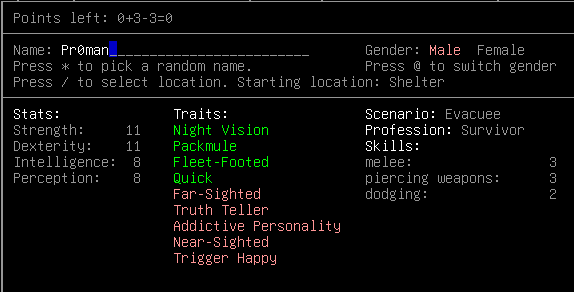
\includegraphics{02}

This would be how our character looks on the finalization screen. So let's hop into the world' is what I'd usually say, but we have some dry stuff regarding the games' story to cover in the next chapter. Don't worry, it's brief.